\subsection{CMOS-Schaltung} % (fold)
\label{sub:CMOS-Schaltung}
\begin{frame}
    \frametitle{CMOS-Schaltung}
    \framesubtitle{}
    \begin{figure}[H]
    \begin{center}
            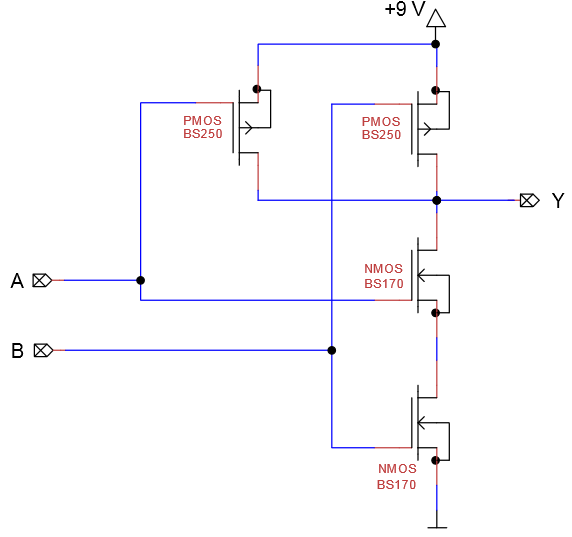
\includegraphics[scale=0.5]{./img/schaltung/1b_cmos.png}
    \end{center}
    \end{figure}    
\end{frame}

\begin{frame}
    \frametitle{CMOS-Schaltung}
    \framesubtitle{}
    \begin{columns}[c]
        \column{0.3\textwidth}
            \begin{center}
                \boxed{
                    \begin{tabular}{c|c||c}
                        A & B & Y \\
                        \hline
                        1 & 0 & 1 \\
                        0 & 1 & 1 \\
                        0 & 0 & 1 \\
                        1 & 1 & 0
                    \end{tabular}
                    }
                \begin{block}{}
                        NAND-Schaltung
                \end{block}
            \end{center}
        \column{0.7\textwidth}
            \begin{figure}[H]
            \begin{center}
                    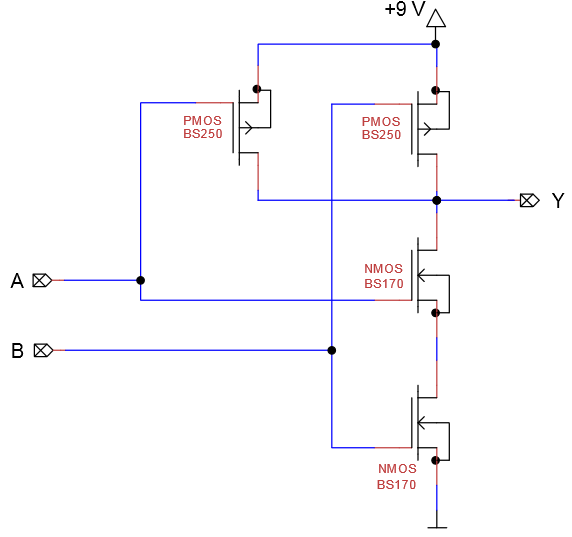
\includegraphics[scale=0.35]{./img/schaltung/1b_cmos.png}
            \end{center}
            \end{figure}    
    \end{columns}
\end{frame}

\begin{frame}
    \frametitle{Funktionsweise}
    \framesubtitle{}
    \begin{block}{}
        \begin{itemize}
            \item PMOS sperren mit H an Basis
            \item NMOS leiten mit H an Basis
        \end{itemize}
    \end{block}
\end{frame}
\begin{frame}
    \frametitle{Funktionsweise}
    \framesubtitle{}
    \begin{columns}[c]
        \column{0.3\textwidth}
            \begin{center}
                \boxed{
                    \begin{tabular}{c|c||c}
                        A & B & Y \\
                        \hline
                        1 & 0 & 1
                    \end{tabular}
                    }
            \end{center}
        \column{0.7\textwidth}
            \begin{figure}[H]
            \begin{center}
                    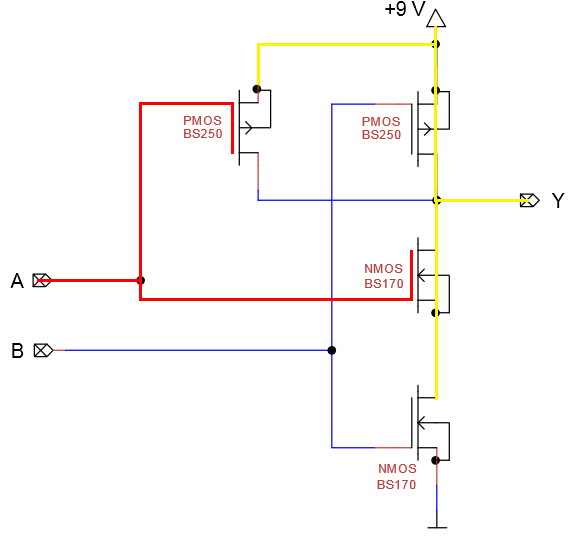
\includegraphics[scale=0.5]{./img/schaltung/cmos_fun_10.png}
            \end{center}
            \end{figure}    
    \end{columns}
\end{frame}
\begin{frame}
    \frametitle{Funktionsweise}
    \framesubtitle{}
    \begin{columns}[c]
        \column{0.3\textwidth}
            \begin{center}
                \boxed{
                    \begin{tabular}{c|c||c}
                        A & B & Y \\
                        \hline
                        1 & 0 & 1 \\
                        0 & 1 & 1 
                    \end{tabular}
                    }
            \end{center}
        \column{0.7\textwidth}
            \begin{figure}[H]
            \begin{center}
                    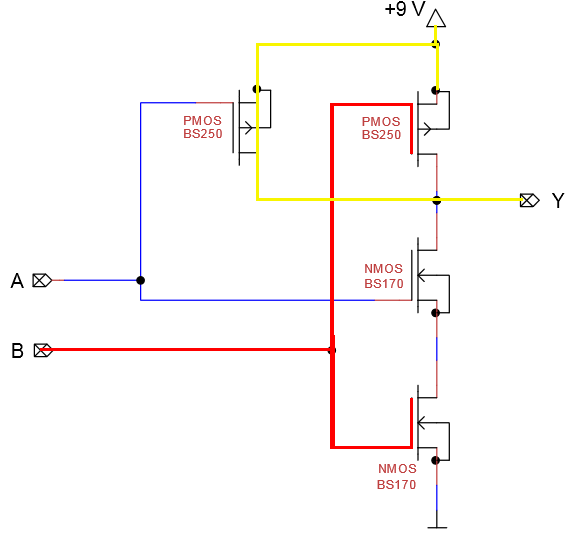
\includegraphics[scale=0.5]{./img/schaltung/cmos_fun_01.png}
            \end{center}
            \end{figure}    
    \end{columns}
\end{frame}
\begin{frame}
    \frametitle{Funktionsweise}
    \framesubtitle{}
    \begin{columns}[c]
        \column{0.3\textwidth}
            \begin{center}
                \boxed{
                    \begin{tabular}{c|c||c}
                        A & B & Y \\
                        \hline
                        1 & 0 & 1 \\
                        0 & 1 & 1 \\
                        0 & 0 & 1
                    \end{tabular}
                    }
            \end{center}
        \column{0.7\textwidth}
            \begin{figure}[H]
            \begin{center}
                    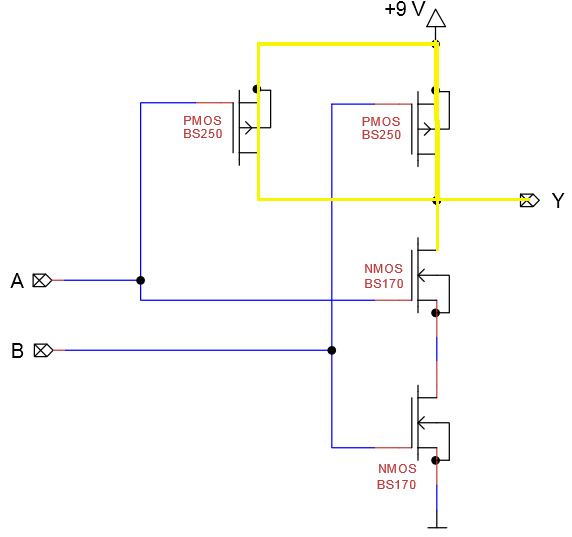
\includegraphics[scale=0.5]{./img/schaltung/cmos_fun_00.png}
            \end{center}
            \end{figure}    
    \end{columns}
\end{frame}
\begin{frame}
    \frametitle{Funktionsweise}
    \framesubtitle{}
    \begin{columns}[c]
        \column{0.3\textwidth}
            \begin{center}
                \boxed{
                    \begin{tabular}{c|c||c}
                        A & B & Y \\
                        \hline
                        1 & 0 & 1 \\
                        0 & 1 & 1 \\
                        0 & 0 & 1 \\
                        1 & 1 & 0
                    \end{tabular}
                    }
            \end{center}
        \column{0.7\textwidth}
            \begin{figure}[H]
            \begin{center}
                    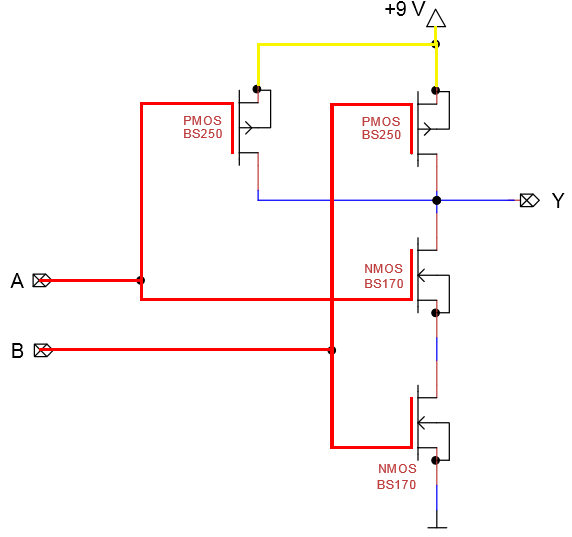
\includegraphics[scale=0.5]{./img/schaltung/cmos_fun_11.png}
            \end{center}
            \end{figure}    
    \end{columns}
\end{frame}
% subsection CMOS-Schaltung (end)
